\documentclass[10pt,Times New Roman]{article}
\usepackage{geometry}
\usepackage{mathptmx}
\usepackage{graphicx}
\usepackage[font=small,labelfont=bf]{caption}
\usepackage{enumitem}


\geometry{a4paper,margin=1in}
\graphicspath{{./graphics/}}


\title{Image Recognition using Deep Learning \\
       American Sign Language}
\author{Zygmunt, Joshua 
        \and
        Watt, Kellen}

\date{December 14, 2018}

\begin{document}
\maketitle
\begin{abstract}
    Hearing loss and hearing impairment are important and debilitating conditions which can
    severely affect and potentially limit the affected individual’s quality of life.
    Additionally, it can require the affected individual to learn a new language by way of
    some dialect of Sign Language. For many, this can be an exceptionally difficult task,
    since it is theoretically just as difficult as learning a new spoken language, with the
    added challenge of a great deal of potential mental and financial stress associated with
    hearing impairment. Our goal was to find a solution that aids in this education process 
    and helps those who need only minor assistance to function as they did prior to their
    impairment. Herein, we propose a solution, in the form of a deep learning system based
    on neural networks, that can recognize American Sign Language alphabet symbols and
    translate them to their text equivalent. Using a convolutional neural network, we were
    able to achieve a reasonably high rate of accuracy on training data ($>95\%$),
    although this was with a high degree of overfitting on a non-representative data set,
    as we will discuss.
\end{abstract}

\section{Introduction}
    Sign language is a means by which the hearing impaired and otherwise nonverbal individuals
    may communicate, and it is often their most efficient method of doing so. The biggest issue
    with this is that, while necessary, it is nonetheless a language, and must be learned as
    such, which is rarely a simple task. Additionally, once the language is learned, simple
    communication with the general public can still be very difficult, since a vast majority
    of the population is not proficient in any dialect of sign language. Although the data are
    sparse, largely outdated, and do not agree on a specific number, most estimates of complete
    or partial hearing loss are significantly less than 0.5\% of the American population, and
    the percentage of American Sign Language users is a bit higher than that estimate but still
    less than 0.5\%. This creates the opportunity for communication
    failures to arise. Granted, most individuals should be able to communicate in written form,
    but this is usually far slower than communicating verbally or pictorially (as in ASL).
    In this work, we approached this problem by applying different types of neural networks
    to recognize symbols from the ASL alphabet, and translate them to their corresponding
    English letters, which could then be used to form words and larger grammatical structures.

\section{Important Definitions}
    \subsection{American Sign Language (ASL)}
        A version of sign language used primarily in America. Note that it is qualified with
        ``American'' because dialects of sign language vary wildly between countries and cultures,
        and this paper deals only with this specific version.

    \subsection{Linear Layer}\label{def:linearlayer}
        A layer of a Neural Network, described by the following equation:
        \[f(x) = xA^T + B\]
        where $x$ is the floating-point numeric input to the function, $A$ is a matrix of
        floating-point values, and $b$ is a floating-point value attached to the layer itself.
        From this point forward, linear layers will be refered to like so:
        \[[m,n]\]
        where $m$ and $n$ are the dimensions of $A$.

    \subsection{Rectified Linear Unit Function (ReLU)}
        An activation function defined as only the positive component of its argument. Formally
        defined as such:
        \[ReLU(x) = max(0,x)\]

    \subsection{Softmax Function}
        A function that takes an un-normalized vector and normalizes it. Defined as such:
        \[Softmax(x)_j = \frac{exp(x_j)}{\sum_{k=1}^K exp(x_k)}\quad for \ j=1,\ldots,K\]
    \subsection{Max pooling}
        Takes the greatest value from a given area and sends it to the next layer. For example,
        Figure \ref{fig:maxpool} shows the max pooling operation for a kernel size of $2\times2$ with
        stride set to 2.The same operation is used for the convolutional neural network in this paper.

        \begin{figure}[h] 
            \centering 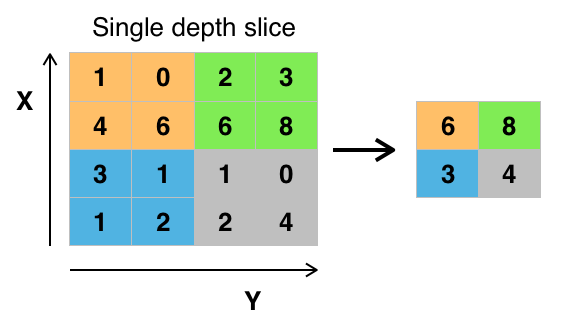
\includegraphics[width=0.5\textwidth]{max_pooling_example}
            \caption{An simple example of max pooling}\label{fig:maxpool}
        \end{figure}

    \subsection{Convolutional Layer}
        A layer in a NN that contains values for a window of area. It multiples those values
        with the overlapping pixels and passes that value on to the next layer, often modified
        by some bias value. This concept is demonstrated in Figure \ref{fig:convlayer}.

        \begin{figure}[h]
            \centering 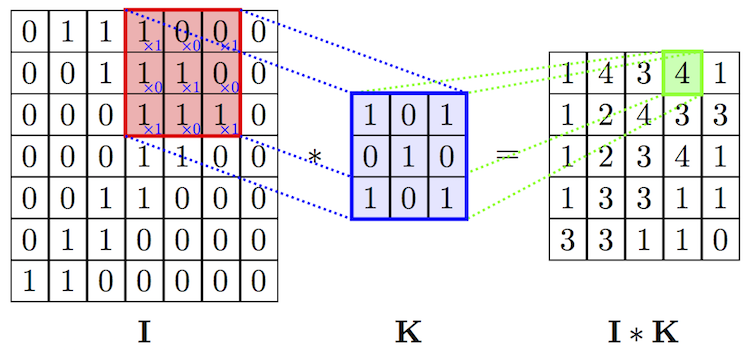
\includegraphics[width=0.5\textwidth]{convolutional_layer_example}
            \caption{An example of how a convolutional layer with kernel size of $3\times3$ and a
                     stide of 1}\label{fig:convlayer}
        \end{figure}

    \subsection{Categorical Entropy Loss}\label{def:catentropyloss}
        A loss function to measure the accuracy of categorization.
        \[loss(x, class) = -log\left(\frac{exp(x[class])}{\sum_j exp(x[j])}\right)\]

    \subsection{One-hot Encoding}
        A bitwise representation of categorical data that requires only one bit to be set and 
        the rest to be cleared. Named as such because only a single bit is ``hot'', or, put more 
        elegantly, there is ``One hot'' bit.

\section{Technical Details}
    \subsection{Data Preprocessing}
    The data used to train the models was originally in the form of $200x200$ JPEG images with 
    three different channels (standard RGB). The images were immediately converted to grayscale, 
    in order to normalize the colors. They were then downsampled to a resolution of $32 \times 32$. At 
    this point, the image has been downscaled from $200 \times 200 \times 3$ to $32 \times 32 \times 1$. 
    An example of this for the letter ``A'' is shown in Figure \ref{fig:a_images}.
 
    \begin{figure}[h]
        \centering {
            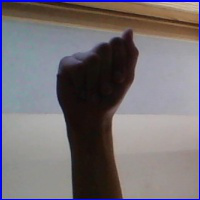
\includegraphics[width=0.25\textwidth]{A_full}
            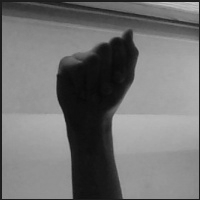
\includegraphics[width=0.25\textwidth]{A_gray}
            
\includegraphics[width=0.25\textwidth]{A_down}
        }
        \caption{Image preprocessing intermediate results}
        \label{fig:a_images}
    \end{figure}
    
    To further simplify the input to the NN, all of these values are divided
    by 255 (the maximum possible value of an individual pixel), and stored in a $32 \times 32$ 
    32-bit floating-point matrix. Additionally, the label of the images is matched to a unique 
    integer value and one-hot encoding vector for training. For example: ``A'' is matched to a value
    of 0, and its one-hot encoding vector (of size 29) is $[1,0,0,\ldots,0]$.

    \subsection{Model Architectures}
    Below are the descriptions of the architectures of the neural networks used for this paper.
    For ease of representation, linear layers will be represented as defined in section 
    \ref{def:linearlayer}. Each element in the lists feeds its results to the next element in
    the same list.

        \subsubsection{Fully Connected Neural Network}
        \begin{itemize}[label=$\rightarrow$]
            \item $[1024, 256]$
            \item ReLU
            \item $[256, 256]$
            \item ReLU
            \item $[256, 29]$
            \item Softmax
        \end{itemize}
      
        \pagebreak
        \subsubsection{Convolutional Neural Network}
        \begin{itemize}[label=$\rightarrow$]
            \item Six convolutional filters $(kernel size=5\times5,\ stride = 1)$ no padding, each biased
            \item ReLU
            \item MaxPool $(kernel size= 2\times2,\ stride = 2)$
            \item $[1260, 1260]$
            \item ReLU
            \item $[1260,29]$
            \item Softmax
        \end{itemize}

    \subsection{Training Information}
        Both models were trained for exactly ten epochs. For each label, there were 3000 
        associated images, which were split into training and testing data sets. The 
        training set contained 90\% of the images, while the testing set contained the
        remaining 10\%. The loss function used was Categorical Entropy Loss (defined in 
        section \ref{def:catentropyloss}). This was applied to the last layer of the network that 
        had no activation function applied. Small batches of size 64 were fed to the model.
        In every epoch, the order of the training set was randomized. Adam was used as the
        optimizer. Before the loss function was used to calculate gradients, it was divided
        by the size of the training set.

    \subsection{Explanation of Design Decisions}
        We chose to use the ASL alphabet, and not a more linguistically complex set of signs
        because this was the most complete, open data source we could readily acquire. We 
        chose to work this since this particular subset of signs is technically sufficient
        to communicate completely, albeit in an inefficient manner. Additionally, it provided
        a complex enough set of classifications to create a proof-of-concept model, which
        could, in theory, be readily extended to include a larger, more-complete set of signs.

        \subsubsection{Side Effects}\label{sec:sideeffects}
            While our decision to use this subset of signs is not unreasonable, the dataset
            we used to train our models was of a poor quality and diversity, which we did
            not realize or even guess until it was far too late to find other data. Our best
            guess for this reason is that source images for each sign were all captured as
            the frames of a video where the creator used the same hand in the same room, and
            simply moved it around to capture unique images.

\section{Results}
    What follows are tables of the results for each model. The final row in each table contains
    the results for each modal at the final experimental epoch.
    \subsection{Fully Connected Neural Network}
    \begin{center}
    \begin{tabular}{|c|c|c|c|}
    \hline
    epoch & epoch loss & training accuracy & test accuracy\\
    \hline
    0&    2.21954766&    0.476922095&    0.467241379\\
    \hline
    1&    1.202423252&    0.617854406&    0.607471264\\
    \hline
    2&    0.864674701&    0.716692209&    0.706666667\\
    \hline
    3&    0.669210446&    0.806807152&    0.794712644\\
    \hline
    4&    0.548182964&    0.81890166&    0.808275862\\
    \hline
    5&    0.463094977&    0.845938697&    0.837816092\\
    \hline
    6&    0.397553019&    0.866947637&    0.862183908\\
    \hline
    7&    0.3456519&    0.85348659&    0.84\\
    \hline
    8&    0.335617101&    0.837126437&    0.824482759\\
    \hline
    9&    0.308817875&    0.913014049&    0.901149425\\
    \hline
    \end{tabular}
    \end{center}

    \subsection{Convolutional Neural Network}
    \begin{center}
    \begin{tabular}{|c|c|c|c|}
        \hline
        epoch&        epoch loss&        training accuracy&        test accuracy\\
        \hline
        0&        1.8721395&        0.69045977&        0.67862069\\
        \hline
        1&        0.7085777&        0.86706258&        0.857931034\\
        \hline
        2&        0.3778454&        0.927458493&        0.919770115\\
        \hline
        3&        0.2374137&        0.950383142&        0.942183908\\
        \hline
        4&        0.1562092&        0.95605364&        0.944712644\\
        \hline
        5&        0.1143182&        0.981111111&        0.978045977\\
        \hline
        6&        0.0854807&        0.982196679&        0.976321839\\
        \hline
        7&        0.0696762&        0.969859515&        0.965402299\\
        \hline
        8&        0.0523054&        0.98853129&        0.982873563\\
        \hline
        9&        0.0425981&        0.98100894&        0.977241379\\
        \hline
    \end{tabular}
    \end{center}


    \subsection{Evaluation of Real-World Test Images}
        While the results of the experiments are very promising, the results of the models
        being applied to external data sources are far less accurate. We suspect this is due
        to the reasons outlined in section \ref{sec:sideeffects}. For example, using the
        real-world image of the ASL sign for ``Y'' in Figure \ref{fig:y_images} led to the classifier
        being sure that it was of the sign for ``P'', which is obviously not correct. A comparison
        of the two is given in Figure \ref{fig:ypcompare} to illustrate the difference.

        \begin{figure}[h]
            \centering {
                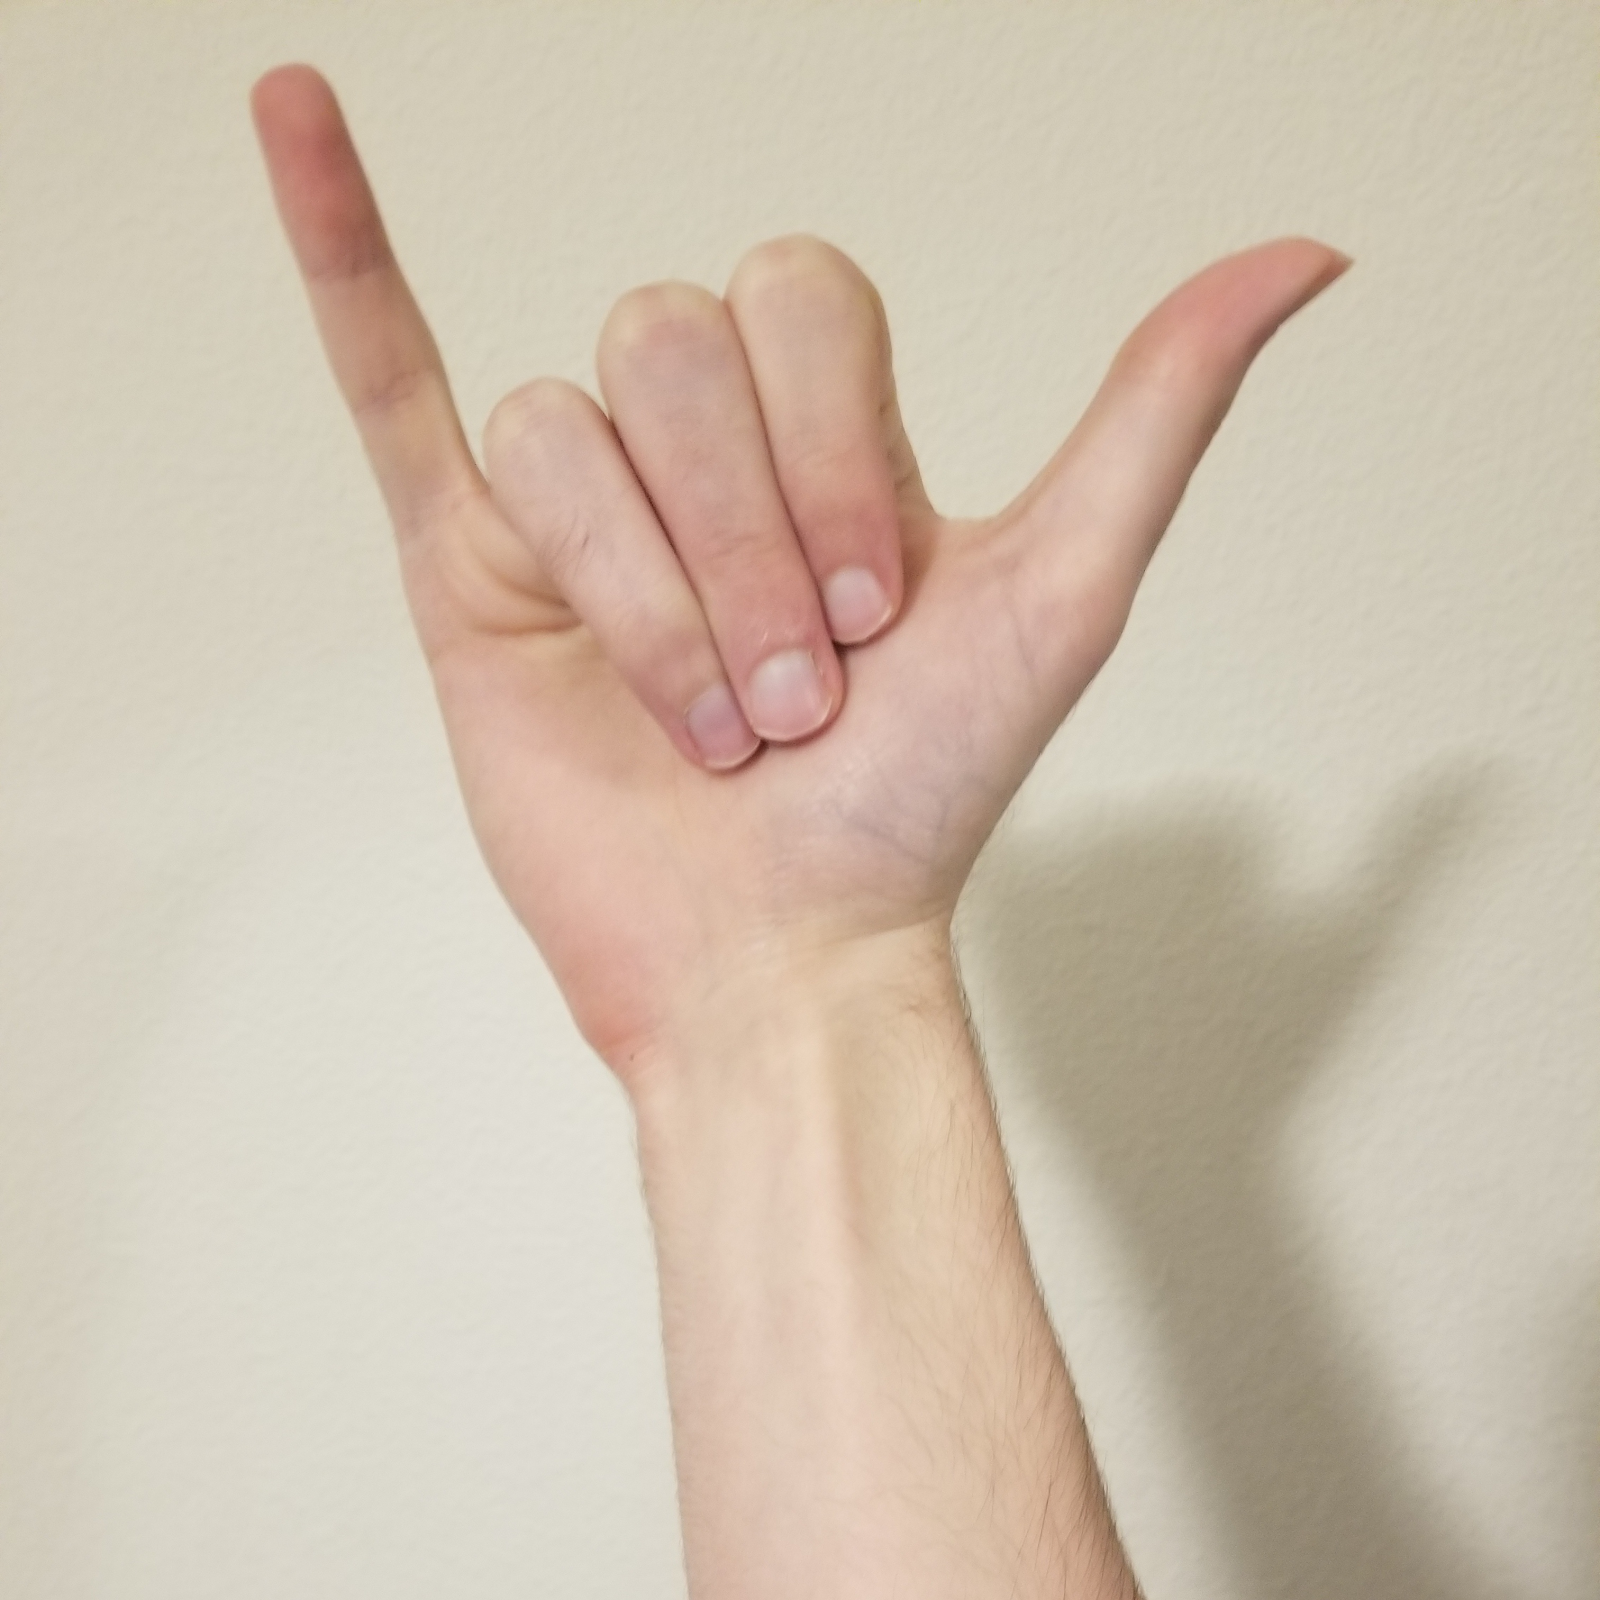
\includegraphics[width=0.25\textwidth]{Y_full}
                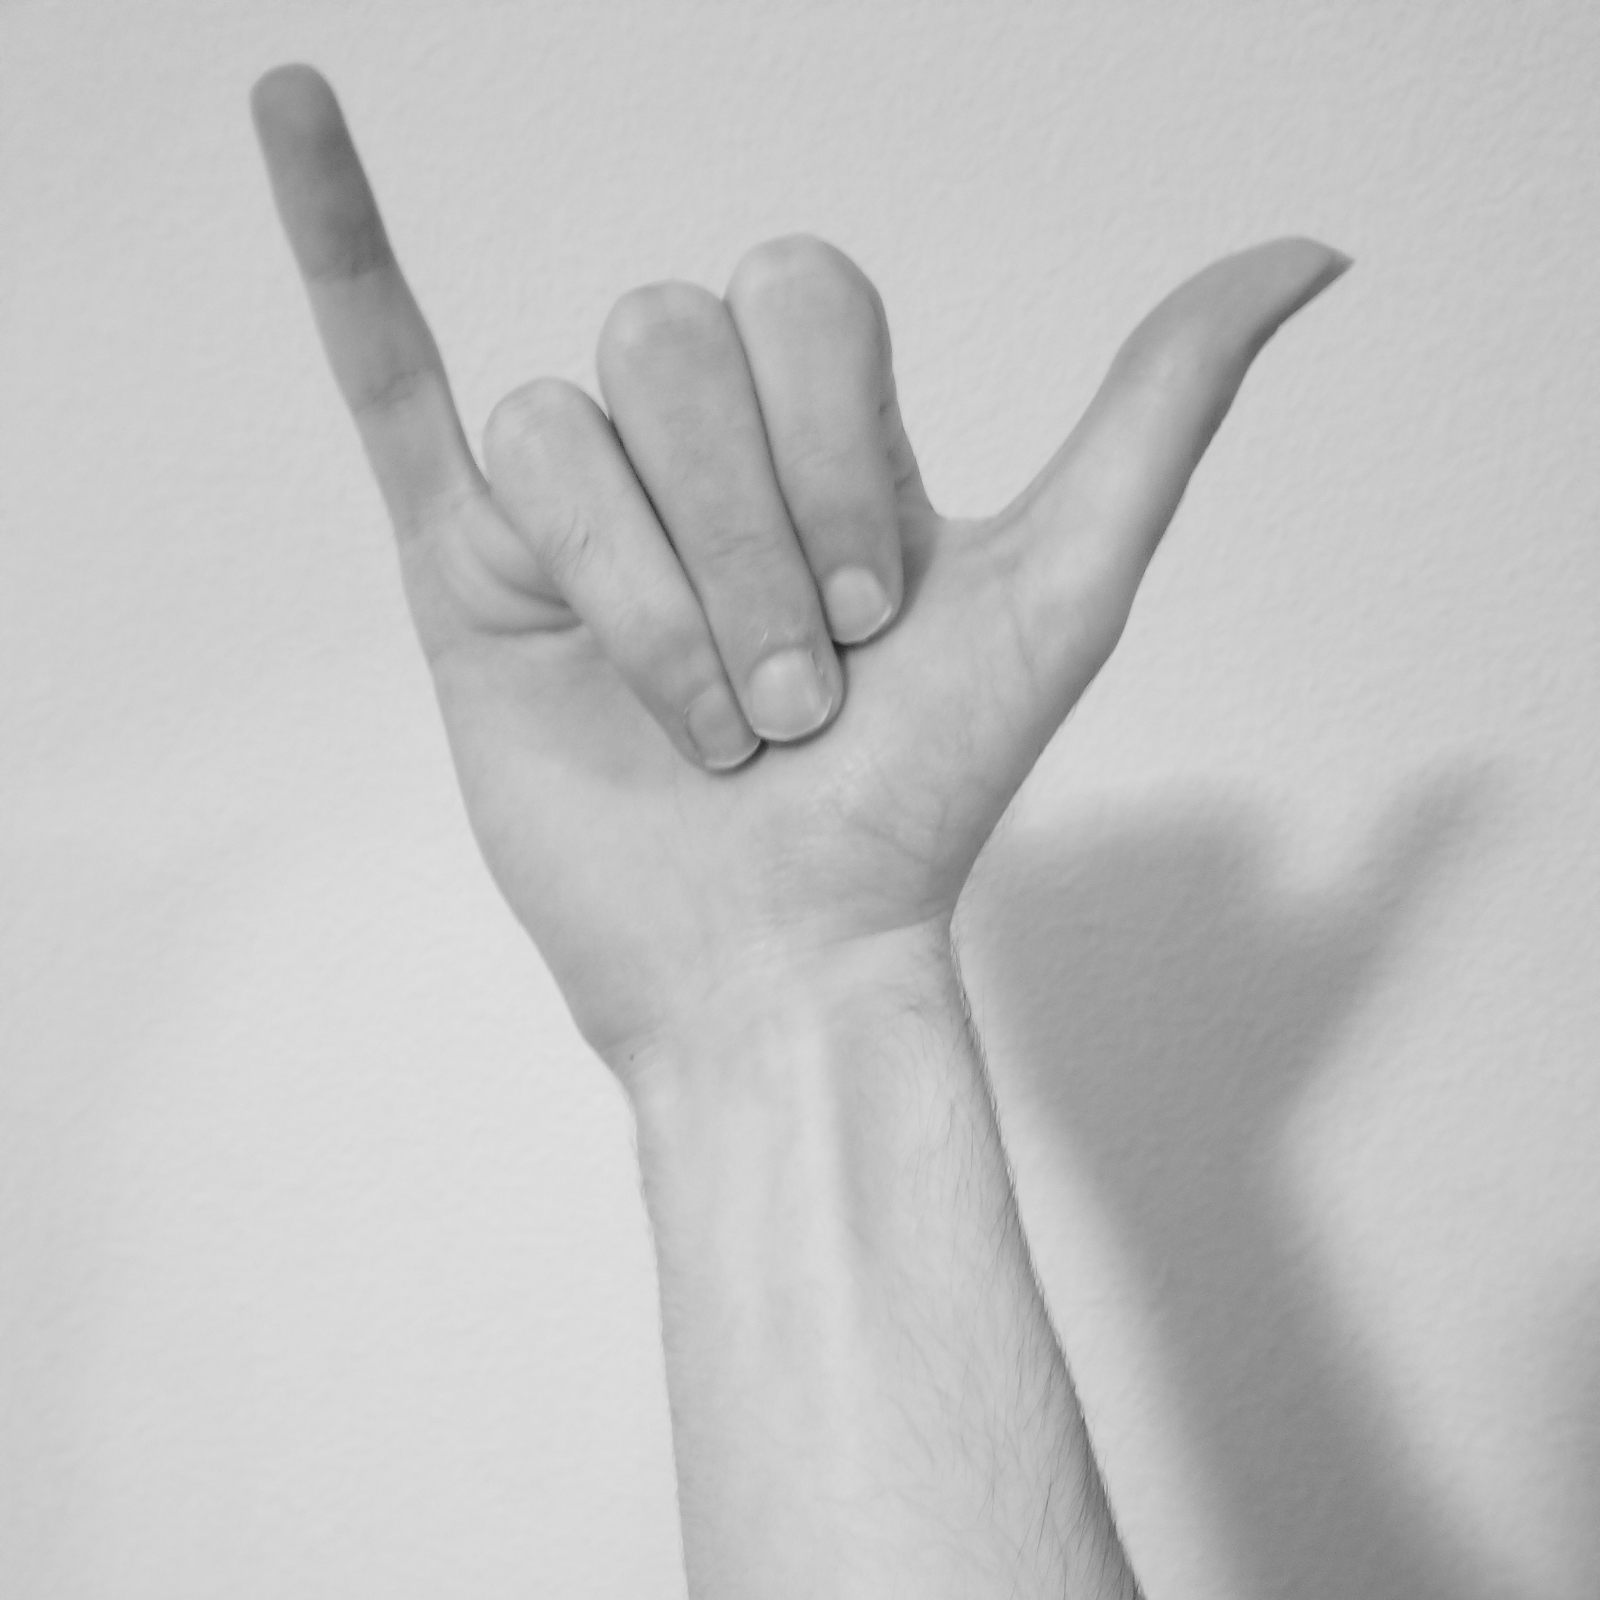
\includegraphics[width=0.25\textwidth]{Y_gray}
                
\includegraphics[width=0.25\textwidth]{Y_down}
            }
            \caption{Real-world testing data for the letter ``Y''}
            \label{fig:y_images}
        \end{figure}

        \begin{figure}[h]
            \centering{
                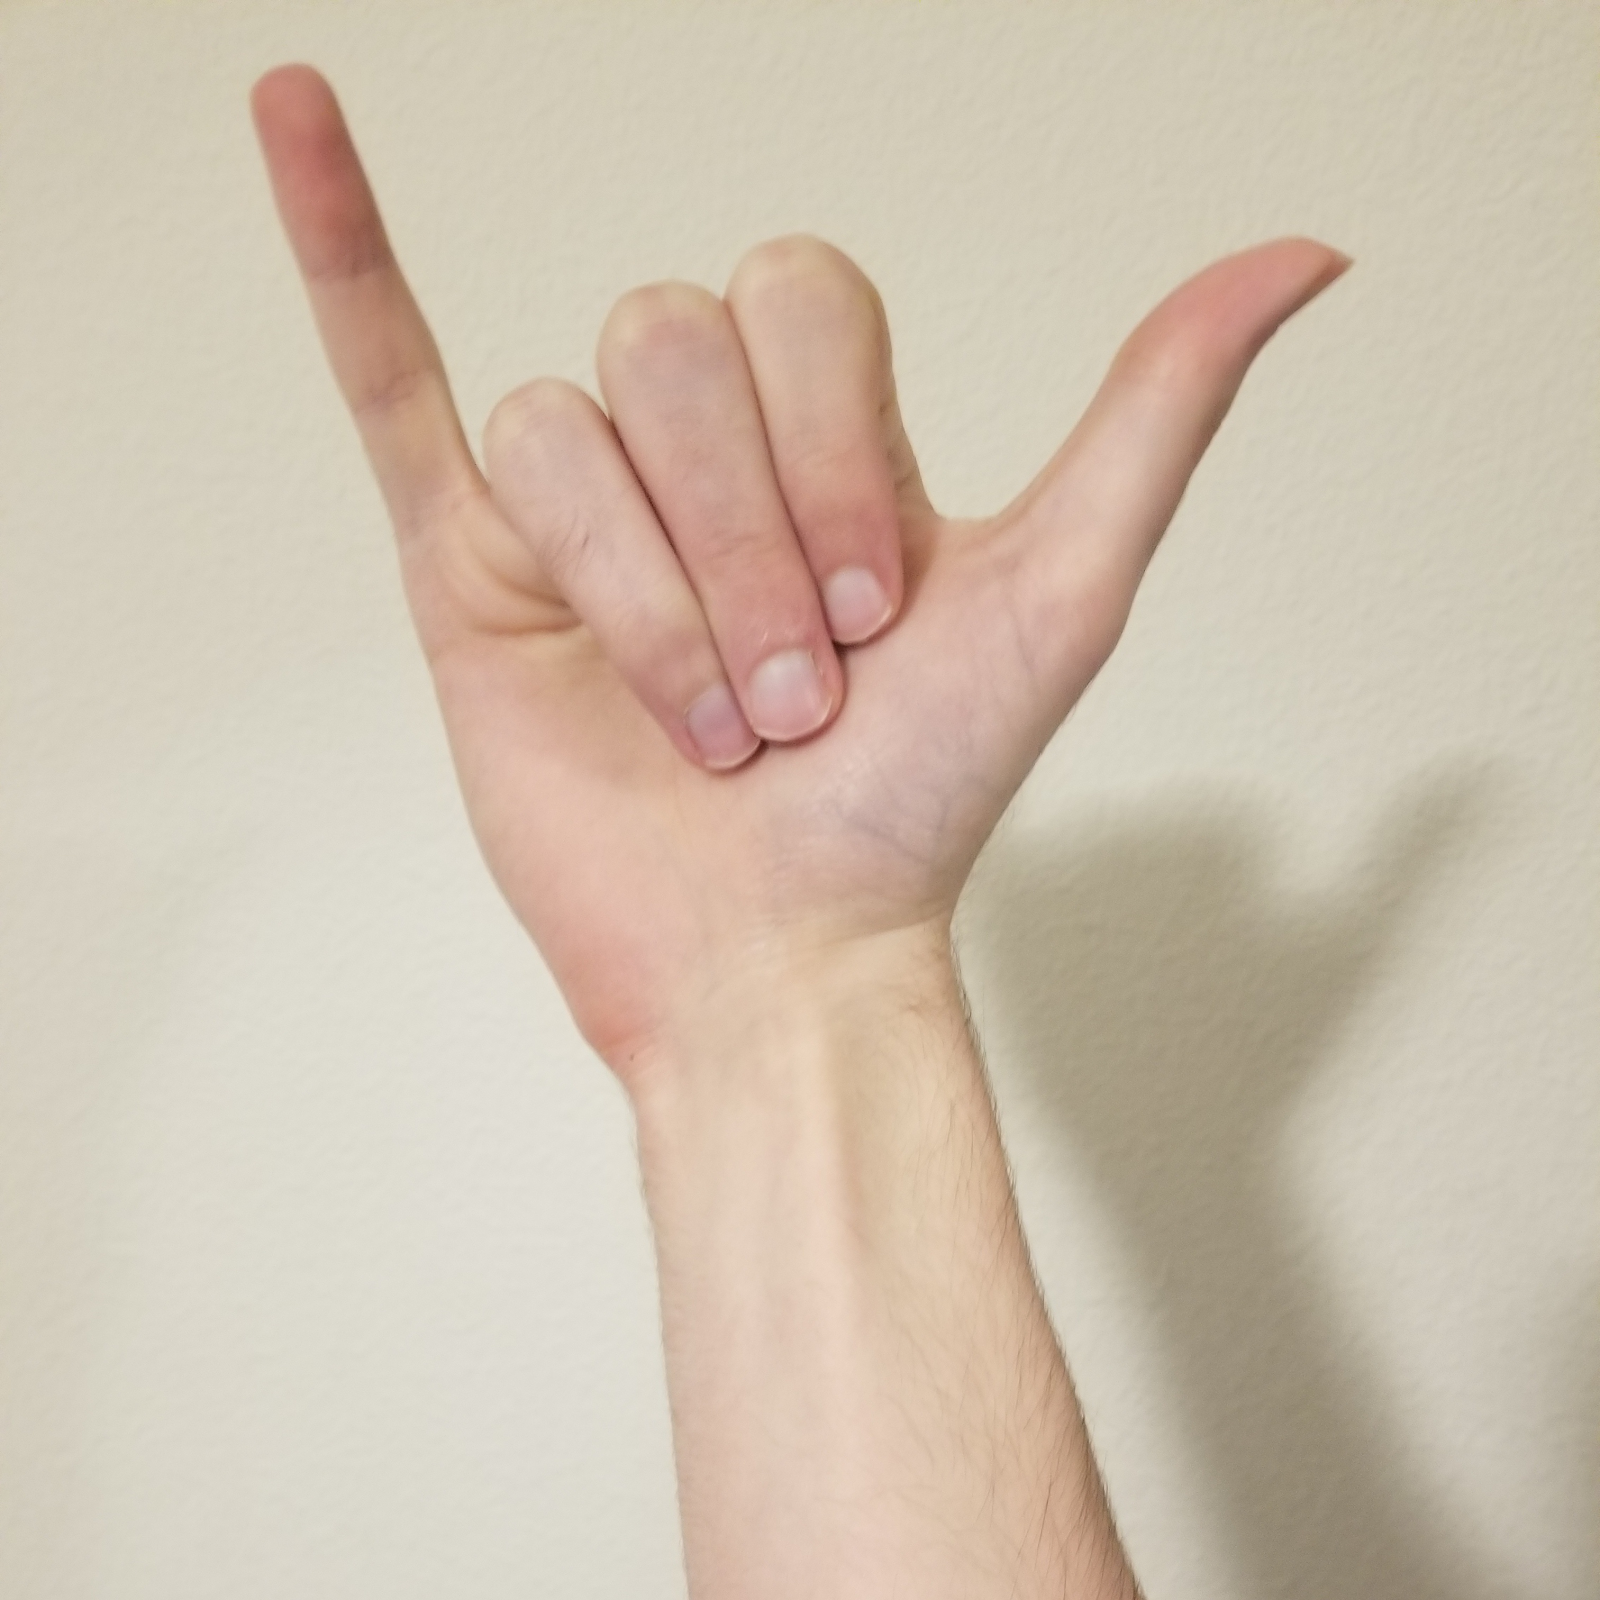
\includegraphics[width=0.25\textwidth]{Y_full}
                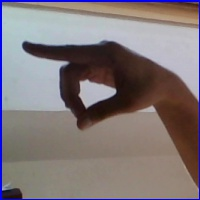
\includegraphics[width=0.25\textwidth]{P_full}
            }
            \caption{The signs for Y and P, respectively}
            \label{fig:ypcompare}
        \end{figure}


\section{Conclusions}
From the results of our experiments, it appears that it is indeed possible and reasonable to
classify, and thus translate ASL signs to their corresponding words. Of course, this is a very
limited study, and significant, albeit relatively simple, changes would be required to make
this system practical for a wider range of signs beyond the alphabet. This is discussed below.
    
    \subsection{Source of Overfitting}
        One of the greatest challenges that faced this project was finding the right classifier,
        as well as finding an appropriate data set. The training data that was used was not at all
        close to diverse enough to represent real-world data, as discussed in Section 
        \ref{sec:sideeffects}. This makes it difficult-to-impossible to classify any sign image that
        was not from that particular data set. In addition to this, there are inherently challanges
        to classifying signs in an image. These include, but are not limited to, the lighting, the
        background, the size of the sign, and the individual hand making the sign, just to name a
        few. Since the training data was so limited, the classifier can not be guaranteed to
        learn a given hand sign from the sign itself, but rather from other environmental
        attributes mentioned. This would lead to the poor performance observed with real-world
        data.

\section{Future Work}
Further directions of study in this vein of research is both required and readily available. 
The first, and most important thing that must done however, is more diverse data must be generated.
Options for this include a custom setup, where we would take images of our own hands in different
settings, with far more variables being changed than in the data used in these experiments. One 
way to achieve this would have been with green-screen technology, where we would replace the green
background with a variety of different backgrounds. Another
option in that regard is crowdsourcing the image-gathering. A benefit is that this could be a 
relatively quick method of gathering images, and the probably dubious quality of the images would
automatically create a great deal of variance, which would greatly help the classifier(s) learn 
properly.

Once the appropriate data is gathered, a possible direction for the research to go would be
refining the models or using more sophisticated models. One such model that seems promising
are Region-based Convolutional Neural Networks (RCNN). This essentially functions by treating
the input image as a set of smaller items which are then individually classified. This appears
to reasonably successful in practice, given that the image is already accompanied by specialized
labels. This was not pursued in this series of experiments because the specialized labels
required more information than we could reasonably require with the time we had.


\end{document}
